\chapter{Kankerbiologie}\label{ch:b3:cancer-biology}

Een \omterm{def:b3:cancer-biology:hallmarks}{tumor} die groot genoeg is om te voelen, een centimeter in
doorsnede, bevat een miljard cellen en is het werk van ongeveer dertig
verdubbelingen vanuit één cel die de verkeerde kant op ging ---
gewoonlijk een decennium groei voordat iemand het wist. Achter die cel
liggen verscheidene mutaties, die elk in dezelfde afstammingslijn
moesten optreden en die elk een van de besturingen van de twee vorige
hoofdstukken weghaalden: een rem op de deling, een trekker van de dood,
een grens aan het aantal delingen, de plicht om te blijven zitten.
\omterm{def:b3:cancer-biology:hallmarks}{Kanker} is de evolutie van een celpopulatie binnen een lichaam, door
mutatie en selectie, naar een toestand die de cellen dient en het
organisme doodt. Dit hoofdstuk behandelt de genen die worden geraakt en
wat zij normaal doen, de statistiek die laat zien hoeveel treffers
nodig zijn, de fysiologie die een \omterm{def:b3:cancer-biology:hallmarks}{tumor} moet verwerven om voorbij een
millimeter te groeien en zich te verspreiden, de oorzaken die te
vermijden zijn, en de behandelingen --- van vergiften die delende
cellen doden tot antilichamen die het afweersysteem loslaten --- die de
biologie mogelijk heeft gemaakt, samen met de evolutionaire reden
waarom zij zo vaak falen.

\section{Wat kanker is}

\begin{definition}[Tumor, kanker, kenmerken]\label{def:b3:cancer-biology:hallmarks}
\index{kanker}\index{tumor}\index{kwaadaardig}\index{metastase}\index{kenmerken van kanker}
Een \emph{tumor} (neoplasma) is een kloon van cellen die aan de
besturing van haar groei is ontsnapt en zich in een weefsel ophoopt.
Hij is \emph{goedaardig} als hij afgebakend en ingekapseld blijft, en
\emph{kwaadaardig} --- een \emph{kanker} --- als zijn cellen naburig
weefsel binnendringen en elders secundaire tumoren stichten (de
\emph{metastase}), en dat is wat doodt. Kankers worden genoemd naar de
cel waaruit zij ontstaan: carcinomen uit epitheel (\qty{85}{\%} van de
menselijke kankers), sarcomen uit bindweefsel, leukemieën en lymfomen
uit bloedvormende cellen, gliomen uit glia. Welk weefsel het ook is,
een kwaadaardige kloon heeft dezelfde reeks vermogens verworven, de
\emph{kenmerken van kanker}: hij deelt zich zonder groeisignalen van
buiten en negeert de signalen die hem zouden stoppen; hij weerstaat de
\omterm{def:b3:cell-cycle-apoptosis:apoptosis}{apoptose}; hij deelt zich onbeperkt, nadat hij het \omterm{def:b3:cancer-biology:telomerase}{telomerase} weer heeft
aangezet; hij lokt bloedvaten uit; hij dringt binnen en zaait uit; en,
daaronder, is zijn genoom onstabiel, herprogrammeert hij zijn
stofwisseling naar de glycolyse zelfs in zuurstof (het Warburg-effect),
trekt hij ontstekingscellen aan die hem helpen, en ontwijkt hij het
afweersysteem. Elk kenmerk is een besturing van normaal weefsel die is
verslagen, en elk is op genen terug te voeren.
\end{definition}

\begin{omfigure}
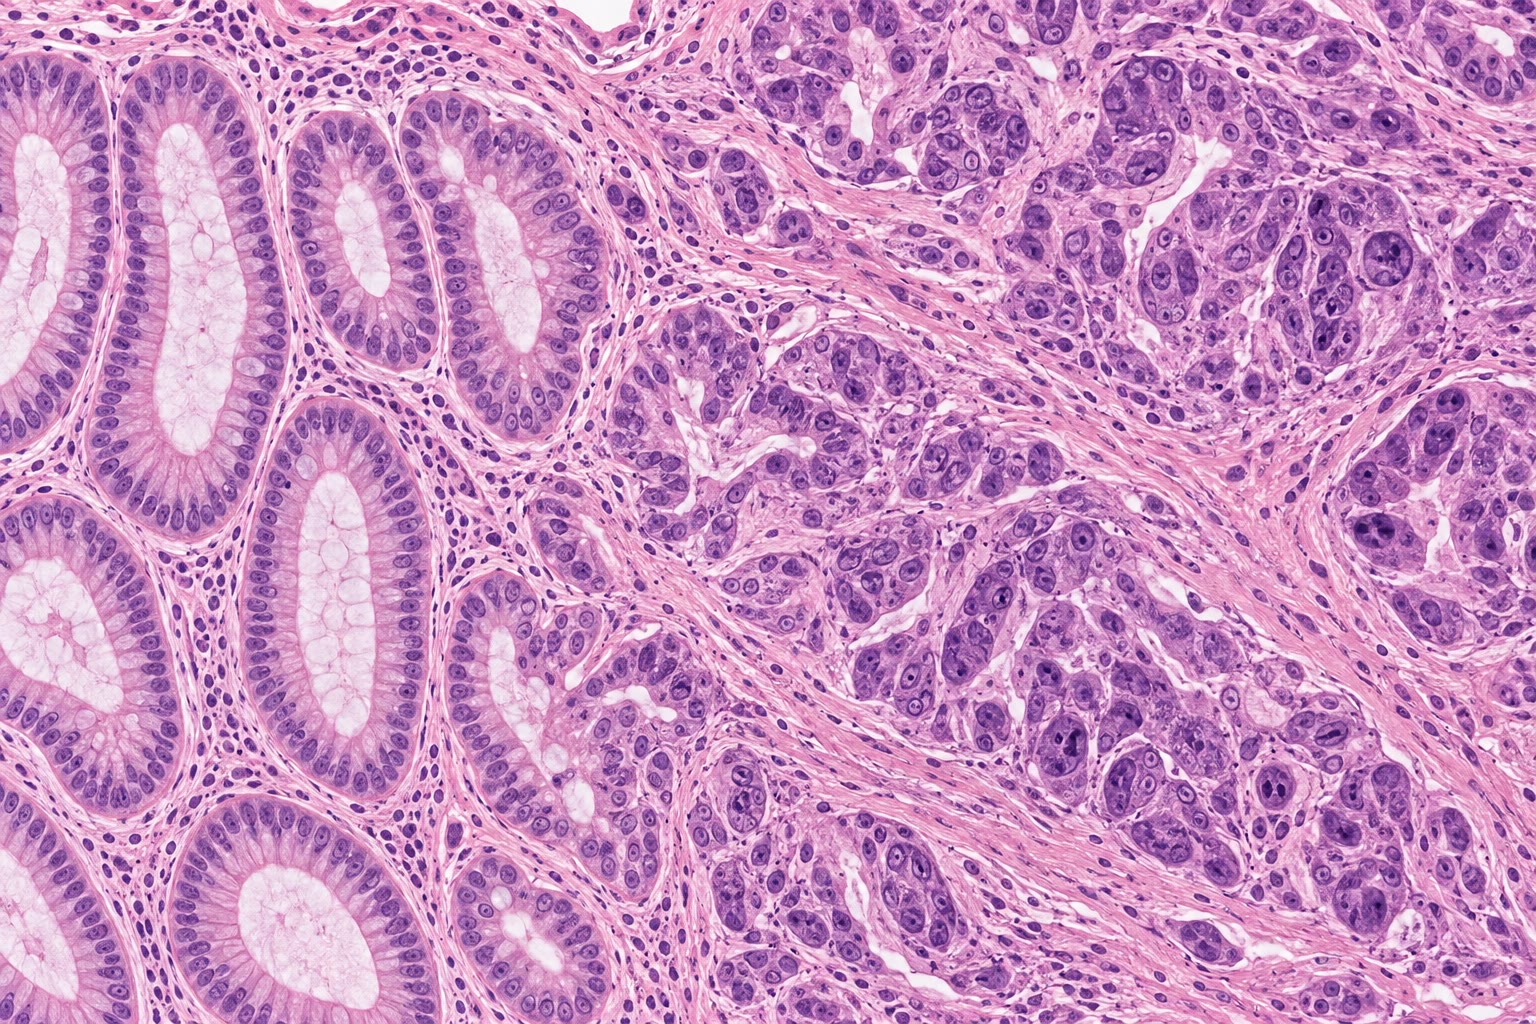
\includegraphics[width=0.56\linewidth]{images/book5/ai/b5-11-tumour-histology.jpg}

{\small Een carcinoom aan zijn grens: links ordelijk klierepitheel met
regelmatige kernen; rechts opeengepakte cellen met grote, onregelmatige
kernen die het onderliggende stroma binnendringen --- het beeld dat een
patholoog leest om een \omterm{def:b3:cancer-biology:hallmarks}{tumor} \omterm{def:b3:cancer-biology:hallmarks}{kwaadaardig} te noemen.}
\end{omfigure}

\section{De genen die worden geraakt}

\begin{definition}[Oncogenen en tumorsuppressoren]\label{def:b3:cancer-biology:genes}
\index{oncogen}\index{proto-oncogen}\index{tumorsuppressorgen}\index{Ras}\index{p53}\index{tweetreffershypothese}
Een \emph{proto-oncogen} is een normaal gen dat de deling of de
overleving bevordert --- een groeifactor, zijn receptor, een
signaaleiwit, een transcriptiefactor, een \omterm{def:b3:cell-cycle-apoptosis:cdk}{cycline} --- en een
\emph{oncogen} is een mutante vorm die werkzaam is zonder zijn normale
signaal: een puntmutatie die het kleine GTPase \emph{Ras} in zijn
GTP-toestand vastzet (glycine~12 in een kwart van alle \omterm{def:b3:cancer-biology:hallmarks}{kankers}), een
vermenigvuldiging van het gen voor de receptor HER2 of voor de
transcriptiefactor Myc, een translocatie die \emph{BCR} aan het kinase
\emph{ABL} versmelt bij chronische myeloïde leukemie of \emph{MYC} naast
een antilichaam-enhancer legt bij het burkittlymfoom. Eén mutant allel
volstaat: oncogenen werken dominant. Een \emph{tumorsuppressorgen}
beteugelt de deling of dwingt dood of herstel af --- Rb en p16 bij het
\omterm{def:b3:cell-cycle-apoptosis:checkpoints}{restrictiepunt}, \emph{p53}, de bewaker die een beschadigde cel stilzet
of doodt, APC in de \omterm{prop:b3:cancer-biology:pathways}{Wnt-route} van de dikke darm, PTEN, BRCA1 en BRCA2,
de genen van het \omterm{prop:b3:dna-repair:fidelity}{mismatchherstel} --- en het moet beide allelen
verliezen om bij te dragen: \emph{twee treffers}, waarvan de eerste bij
de familiaire kankersyndromen vaak wordt geërfd en de tweede somatisch
is. \emph{p53} is bij de helft van alle menselijke \omterm{def:b3:cancer-biology:hallmarks}{kankers} gemuteerd en
zijn route bij de meeste overige uitgeschakeld.
\end{definition}

\begin{proof}[Bewijsmateriaal]
Rous (1911) bracht een kippensarcoom over met een celvrij filtraat, een
virus, waarvan het enkele transformerende gen, \emph{src}, door Varmus
en Bishop (1976) een gekaapte kopie van een normaal kippengen bleek te
zijn --- \omterm{def:b3:cancer-biology:genes}{oncogenen} zijn gewijzigde cellulaire genen. Weinberg (1982)
bracht DNA uit een menselijk blaascarcinoom over in gekweekte
muizencellen, die getransformeerd raakten; het verantwoordelijke
fragment was \emph{RAS} met één basenverandering, en diezelfde
verandering ontbrak in het normale weefsel van de patiënt. Knudson
(1971) vergeleek kinderen met de oogtumor retinoblastoom: wie een
familiegeschiedenis had kreeg vroeg verscheidene \omterm{def:b3:cancer-biology:hallmarks}{tumoren} in beide ogen;
wie die niet had kreeg er later één --- passend bij familiaire gevallen
die één somatische gebeurtenis nodig hebben en sporadische die er twee
nodig hebben, en dus bij een gen waarvan beide kopieën verloren moeten
gaan. \emph{RB} werd in 1986 gekloneerd, en beide allelen bleken in
elke \omterm{def:b3:cancer-biology:hallmarks}{tumor} inderdaad uitgeschakeld.
\end{proof}

\begin{theorem}[Treffers en de leeftijdscurve]\label{thm:b3:cancer-biology:armitage-doll}
\index{model van Armitage--Doll}\index{meerstapscarcinogenese}
Stel dat een \omterm{def:b3:cancer-biology:hallmarks}{kanker} $k$ onafhankelijke, snelheidsbepalende
gebeurtenissen in één cellijn vergt, die elk met een constante snelheid
$u$ per cel per jaar optreden, in een populatie van $N$ vatbare cellen,
met $ut \ll 1$. Dan is de kans dat een gegeven cel alle $k$
gebeurtenissen op leeftijd $t$ heeft doorgemaakt ongeveer $(ut)^{k}$, is het
cumulatieve risico in het weefsel ongeveer $N(ut)^{k}$, en is de
incidentie --- nieuwe gevallen per jaar op leeftijd $t$ ---
\[
I(t) \approx N\,k\,u^{k}\,t^{\,k-1},
\]
een macht van de leeftijd met exponent $k - 1$: een rechte lijn met
helling $k - 1$ op een dubbellogaritmische grafiek. Voor iemand die een
van de gebeurtenissen erft heeft dezelfde \omterm{def:b3:cancer-biology:hallmarks}{kanker} een incidentie
$\propto t^{\,k-2}$, één macht lager.
\end{theorem}
\begin{proof}
Elke gebeurtenis, met snelheid $u$, heeft zich vóór tijdstip $t$
voorgedaan met kans $1 - e^{-ut} \approx ut$; de gebeurtenissen zijn
onafhankelijk, dus hebben alle $k$ zich voorgedaan met kans
$(ut)^{k}$, en de volgorde waarin dat gebeurde doet hier niet ter zake.
Met $N$ cellen en zeldzame gebeurtenissen is het verwachte aantal
cellen dat de reeks heeft voltooid $N(ut)^{k}$, en de incidentie is de
afgeleide daarvan naar de tijd, $Nku^{k}t^{k-1}$. Wie één gebeurtenis
erft houdt er $k - 1$ over: $(ut)^{k-1}$, incidentie $\propto t^{k-2}$.
Deed de volgorde van de gebeurtenissen ertoe (slechts $1$ van de $k!$
volgordes leidde tot \omterm{def:b3:cancer-biology:hallmarks}{kanker}), dan zou de voorfactor veranderen, niet de
exponent.
\end{proof}

\begin{example}[De exponent lezen]\label{ex:b3:cancer-biology:exponent}
De incidentie van de meeste carcinomen bij volwassenen stijgt als
ongeveer de vijfde tot zesde macht van de leeftijd --- van ongeveer $1$
op \num{100000} per jaar op dertigjarige leeftijd tot $1$ op $300$ op
tachtigjarige, een factor $300$ voor een factor $2.7$ in leeftijd, en
$2.7^{5.7} \approx 300$ --- wat op zes of zeven snelheidsbepalende
gebeurtenissen wijst. De schatting is grof: de uitbreiding van een
kloon na elke treffer verhoogt het aantal cellen dat de volgende loopt,
zodat minder gebeurtenissen met klonale groei ertussen dezelfde helling
geven, en het aantal \emph{aandrijvende} mutaties in gesequencede
\omterm{def:b3:cancer-biology:hallmarks}{tumoren} is twee tot acht. Het retinoblastoom van Knudson past precies
bij de tweede uitspraak van de stelling: de sporadische ziekte, die
twee treffers vergt, heeft een incidentie die met de leeftijd stijgt
(gedurende de paar jaar dat de retinoblasten bestaan); de erfelijke
ziekte, die er één vergt, is vanaf de geboorte met vrijwel constante
snelheid aanwezig en slaat vroeg en herhaaldelijk toe.
\end{example}

\begin{omfigure}
\begin{tikzpicture}
\begin{axis}[
  width=0.68\linewidth, height=6cm,
  xmode=log, ymode=log,
  xmin=20, xmax=100, ymin=1e-6, ymax=1e-1,
  xlabel={leeftijd (jaren)}, ylabel={incidentie per persoon per jaar},
  xlabel style={font=\small, at={(axis description cs:0.5,-0.12)}, anchor=north},
  ylabel style={font=\small},
  tick label style={font=\small}, xtick={20,30,50,80}, xticklabels={20,30,50,80},
  clip=false,
]
\addplot[very thick, omThm, domain=20:100, samples=2] {1e-5*(x/30)^5.7};
\addplot[very thick, omDef, domain=20:100, samples=2] {3e-4*(x/30)^1};
\addplot[very thick, omMeth!70!black, domain=20:100, samples=2] {2e-3};
\node[font=\scriptsize, omThm, anchor=south west] at (axis cs:38,2.5e-6) {carcinomen: helling $5$--$6$, zes of zeven gebeurtenissen};
\node[font=\scriptsize, omDef, anchor=south west] at (axis cs:22,6e-4) {twee treffers: helling 1};
\node[font=\scriptsize, omMeth!70!black, anchor=south west] at (axis cs:22,2.3e-3) {één treffer geërfd: helling 0};
\end{axis}
\end{tikzpicture}

{\small Incidentie tegen leeftijd op logaritmische assen. Een \omterm{def:b3:cancer-biology:hallmarks}{kanker}
die $k$ snelheidsbepalende gebeurtenissen vergt stijgt als $t^{k-1}$:
de steile lijn van de carcinomen bij volwassenen, en de twee gevallen
van Knudson --- een \omterm{def:b3:cancer-biology:hallmarks}{tumor} met twee treffers die lineair stijgt, en
dezelfde \omterm{def:b3:cancer-biology:hallmarks}{tumor} bij een drager van één geërfde treffer, met een
constante snelheid vanaf de geboorte.}
\end{omfigure}

\begin{proposition}[De routes die worden geraakt]\label{prop:b3:cancer-biology:pathways}
\index{Ras-MAPK-route}\index{PI3K-route}\index{Wnt-route}
De honderden kankergenen vallen in een tiental routes uiteen, die een
\omterm{def:b3:cancer-biology:hallmarks}{tumor} elk ergens uitschakelt. De groeifactorroutes: een
receptortyrosinekinase (EGFR, HER2), \omterm{def:b3:cancer-biology:genes}{Ras}, de kinasecascade
Raf--MEK--ERK naar de kern, en daarnaast PI3K--Akt--mTOR richting
overleving en groei, beteugeld door PTEN; een \omterm{def:b3:cancer-biology:hallmarks}{tumor} zet er een van aan,
door welk gen dan ook. De rem op de \omterm{def:b3:cell-cycle-apoptosis:cdk}{celcyclus}: \omterm{def:b3:cell-cycle-apoptosis:cdk}{cycline} D, Cdk4, p16, Rb
(\cref{ch:b3:cell-cycle-apoptosis}). De bewaker: \omterm{def:b3:cancer-biology:genes}{p53} en zijn
regulatoren. De dood: Bcl-2. De signalering van de ontwikkeling: Wnt
(APC, $\beta$-catenine) in de dikke darm, Hedgehog in huid en hersenen,
Notch in T-cellen. Het onderhoud van het genoom: het \omterm{prop:b3:dna-repair:fidelity}{mismatchherstel},
\omterm{def:b3:dna-repair:dsb}{BRCA}, \omterm{def:b3:dna-repair:ddr}{ATM}. Het \omterm{def:b3:chromatin-epigenetics:nucleosome}{chromatine}: de \omterm{def:b3:chromatin-epigenetics:histone-code}{schrijvers} en verbouwers van
\cref{ch:b3:chromatin-epigenetics}, gemuteerd in een derde van de
\omterm{def:b3:cancer-biology:hallmarks}{tumoren}. De onsterfelijkheid: de promotor van het \omterm{def:b3:cancer-biology:telomerase}{telomerase}. Omdat een
route een reeks stappen is, zijn mutaties in verschillende genen
alternatieven --- een \omterm{def:b3:cancer-biology:hallmarks}{tumor} met mutant \omterm{def:b3:cancer-biology:genes}{Ras} heeft zelden ook mutant EGFR
--- en kunnen geneesmiddelen tegen de ene stap door een mutatie
stroomafwaarts worden verslagen.
\end{proposition}

\begin{omfigure}
\begin{tikzpicture}[every node/.style={font=\scriptsize}, >=stealth]
  % membrane
  \draw[very thick, omDef] (0,3.6) -- (12,3.6); \draw[very thick, omDef] (0,3.3) -- (12,3.3);
  \node[above] at (1.0,3.65) {buiten}; \node[below] at (1.0,3.25) {cytosol};
  % receptor
  \draw[thick, fill=omProp!35] (3.7,3.0) rectangle (4.1,4.1); \draw[thick, fill=omProp!35] (4.3,3.0) rectangle (4.7,4.1);
  \node[above, align=center] at (4.2,4.15) {groeifactor $\to$ receptorkinase\\(EGFR, HER2)}; \node[right, omThm, font=\tiny] at (4.75,4.0) {vermenigvuldigd};
  % Ras
  \node[draw, thick, rounded corners, fill=omDef!20] (ras) at (4.2,2.3) {Ras--GTP};
  \node[right, omThm, font=\tiny] at (5.0,2.3) {G12: altijd aan};
  \node[draw, thick, rounded corners, fill=omDef!20] (raf) at (4.2,1.4) {Raf $\to$ MEK $\to$ ERK};
  \node[right, omThm, font=\tiny] at (5.8,1.4) {BRAF V600E};
  \node[draw, thick, rounded corners, fill=omMeth!25] (myc) at (4.2,0.4) {Myc, cycline D: deling};
  \node[right, omThm, font=\tiny] at (6.4,0.4) {Myc vermenigvuldigd};
  \draw[->, thick] (4.2,3.0) -- (ras); \draw[->, thick] (ras) -- (raf); \draw[->, thick] (raf) -- (myc);
  % PI3K branch
  \node[draw, thick, rounded corners, fill=omDef!20] (pi3k) at (9.6,2.3) {PI3K $\to$ Akt $\to$ mTOR};
  \node[draw, thick, rounded corners, fill=omMeth!25] (surv) at (9.6,0.4) {overleving, groei};
  \draw[->, thick] (4.7,3.0) .. controls (6.5,2.8) .. (pi3k.north west); \draw[->, thick] (pi3k) -- (surv);
  \node[draw, thick, rounded corners, fill=omThm!15] (pten) at (12.2,1.4) {PTEN}; \draw[-|, thick, omThm] (pten) -- (9.6,1.4);
  \node[below, omThm, font=\tiny] at (12.2,1.15) {verwijderd};
  % p53 and Rb on the side
  \node[draw, thick, rounded corners, fill=omThm!15] (rb) at (1.2,0.4) {Rb, p16}; \draw[-|, thick, omThm] (rb) -- (myc);
  \node[below, omThm, font=\tiny, align=center] at (1.2,0.15) {beide allelen verloren};
  \node[draw, thick, rounded corners, fill=omThm!15] (p53) at (1.2,1.6) {p53}; \node[below, omThm, font=\tiny, align=center] at (1.2,1.35) {gemuteerd in de helft\\van de kankers};
  \draw[-|, thick, omThm] (p53) -- (1.2,0.65);
\end{tikzpicture}

{\small De groeifactorroutes en waar \omterm{def:b3:cancer-biology:hallmarks}{kankers} erop inslaan. De groene
vakken zijn de uitkomsten, de blauwe de signaalstappen die oncogene
mutaties aan zetten, de rode de suppressoren die \omterm{def:b3:cancer-biology:hallmarks}{tumoren} verliezen (de
balken duiden remming aan). Een \omterm{def:b3:cancer-biology:hallmarks}{tumor} draagt doorgaans één activerende
en een of twee uitschakelende beschadigingen in dit schema.}
\end{omfigure}

\section{Een tumor evolueert}

\begin{proposition}[Carcinogenese in meer stappen]\label{prop:b3:cancer-biology:multistep}
\index{aandrijvende mutatie}\index{meelifterende mutatie}\index{klonale evolutie}\index{mutatiehandtekening}
Een \omterm{def:b3:cancer-biology:hallmarks}{tumor} is het product van somatische evolutie: mutatie brengt
varianten voort, en de selectie binnen het weefsel bevoordeelt die
welke zich meer delen, minder sterven of aan een beperking ontsnappen.
De colorectale reeks die Vogelstein uitzocht is het voorbeeld: het
verlies van \emph{APC} geeft een kleine goedaardige poliep; een mutatie
in \emph{KRAS} laat die tot een adenoom uitgroeien; het verlies van
\emph{SMAD4} of \emph{TP53} maakt er een carcinoom van; verdere
veranderingen maken \omterm{def:b3:cancer-biology:metastasis}{invasie} mogelijk. Elke stap is een klonale
uitbreiding die het aantal cellen vermenigvuldigt dat de volgende
loopt. Een gesequencede \omterm{def:b3:cancer-biology:hallmarks}{tumor} draagt duizenden mutaties, waarvan een
handvol --- doorgaans twee tot acht --- \emph{aandrijvers} zijn die
selectief voordeel gaven; de rest zijn \emph{meelifters}, meegevoerd in
de kloon, en hun spectrum is een verslag van wat hen veroorzaakte:
C$\to$T bij naburige pyrimidines door ultraviolet licht bij het
melanoom, G$\to$T door tabaksrook bij longkanker, de vingerafdrukken
van de APOBEC-enzymen, van gebrekkig \omterm{prop:b3:dna-repair:fidelity}{mismatchherstel}, van aflatoxine
--- de \emph{mutatiehandtekeningen}. \omterm{def:b3:cancer-biology:hallmarks}{Tumoren} zijn heterogeen, een
vertakkende boom van subklonen, en de subkloon die doodt is bij de
diagnose vaak een minderheid.
\end{proposition}

\begin{omfigure}
\begin{tikzpicture}[every node/.style={font=\scriptsize}, >=stealth]
  \foreach \x/\lab/\gene/\col/\r in {0/normaal epitheel/{}/omDef!20/0.5, 2.6/kleine poliep/{APC verloren (beide allelen)}/omDef!35/0.7, 5.4/adenoom/{KRAS geactiveerd}/omProp!40/1.0, 8.4/carcinoom/{SMAD4 of TP53 verloren}/omThm!35/1.3, 11.6/{invasief, uitgezaaid}/{verdere aandrijvers,\\instabiliteit}/omThm!60/1.5} {
    \draw[thick, fill=\col] (\x,0) circle (\r);
    \node[below, align=center] at (\x,-1.6) {\lab};
    \node[above, align=center, omThm] at (\x,1.6) {\gene};
  }
  \foreach \a/\b in {0.5/1.9, 3.3/4.4, 6.4/7.1, 9.7/10.1} \draw[->, very thick] (\a,0) -- (\b,0);
  \node[below] at (5.8,-2.3) {tien tot dertig jaar; elke stap een klonale uitbreiding die het aantal cellen vermenigvuldigt dat de volgende loopt};
\end{tikzpicture}

{\small De colorectale reeks. Elke \omterm{prop:b3:cancer-biology:multistep}{aandrijvende mutatie} breidt een kloon
uit, en de uitgebreide kloon levert de cellen waarin de volgende
aandrijver kan ontstaan; de hele weg kost decennia, en daarom voorkomt
het opsporen van poliepen de \omterm{def:b3:cancer-biology:hallmarks}{kanker}.}
\end{omfigure}

\begin{method}[De amestest]\label{met:b3:cancer-biology:ames}
\index{amestest}\index{mutageen}
Om te toetsen of een stof mutageen is, en dus waarschijnlijk
kankerverwekkend: (1) neem een stam van \emph{Salmonella} met een
puntmutatie in een gen voor de biosynthese van histidine, die zonder
histidine niet kan groeien; (2) meng de stof met een leverextract,
waarvan de enzymen veel verbindingen in hun werkzame mutagene vormen
omzetten zoals het lichaam dat zou doen; (3) breng zo'n $10^{8}$
bacteriën met het mengsel uit op agar zonder histidine; (4) tel de
kolonies die groeien --- elk is een revertant waarin een nieuwe mutatie
het gen heeft hersteld; (5) vergelijk met de spontane snelheid. Een
dosisafhankelijke toename van revertanten betekent dat de verbinding
puntmutaties veroorzaakt. De meeste bekende carcinogenen zijn positief;
de test is goedkoop, duurt twee dagen, en een verbinding die erdoor
valt wordt verder onderzocht voordat zij wordt gemaakt.
\end{method}

\begin{definition}[Onsterfelijkheid en instabiliteit]\label{def:b3:cancer-biology:telomerase}
\index{telomerase}\index{chromosomale instabiliteit}\index{aneuploïdie!bij kanker}
Normale somatische cellen missen telomerase en tellen hun delingen in
de lengte van hun telomeren (\cref{ch:b3:stem-cells}): na een stuk of
vijftig gaan zij in \omterm{def:b3:cell-cycle-apoptosis:other}{senescentie}, en een cel die de \omterm{def:b3:cell-cycle-apoptosis:other}{senescentie} omzeilt
door \omterm{def:b3:cancer-biology:genes}{p53} en Rb te verliezen gaat door tot haar telomeren op zijn en
haar chromosomen versmelten en breken --- een crisis die de meeste
klonen doodt. De zeldzame overlevende heeft het \emph{telomerase} weer
aangezet, meestal door een mutatie in de promotor, en is onsterfelijk;
\qty{90}{\%} van de \omterm{def:b3:cancer-biology:hallmarks}{kankers} brengt het enzym tot expressie. De crisis
laat littekens na: versmolten en gebroken chromosomen,
vermenigvuldigingen, deleties, translocaties --- de \emph{chromosomale
instabiliteit}, die, met het verlies van het \omterm{def:b3:cell-cycle-apoptosis:checkpoints}{controlepunt van de
spoelfiguur} en van de reactie van \omterm{def:b3:cancer-biology:genes}{p53} op een verkeerde verdeling, de
meeste vaste \omterm{def:b3:cancer-biology:hallmarks}{tumoren} aneuploïd maakt en hen varianten laat blijven
maken. Een minderheid van de \omterm{def:b3:cancer-biology:hallmarks}{tumoren} heeft in plaats daarvan een
mutatorfenotype door verloren \omterm{prop:b3:dna-repair:fidelity}{mismatchherstel}, met een normaal karyotype
en een duizendvoudige snelheid van puntmutaties.
\end{definition}

\section{De tumor als weefsel}

\begin{proposition}[Zuurstof bepaalt de omvang van een tumor zonder vaten]\label{prop:b3:cancer-biology:oxygen}
\index{angiogenese}\index{diffusiegrens}\index{hypoxie}
Beschouw weefsel dat zuurstof verbruikt met een constante snelheid $q$
per volume-eenheid, aangevoerd door diffusie (coëfficiënt $D$) vanuit
een vat waar de concentratie aan de wand $c_{0}$ is. In één dimensie
geldt in evenwicht $D\,
\mathrm{d}^{2}c/\mathrm{d}x^{2} = q$, dus $c(x) = c_{0} - qx^{2}/2D$,
en raakt de zuurstof op bij de afstand
\[
L = \sqrt{\frac{2Dc_{0}}{q}} .
\]
Met $D = \qty{2e-9}{m^2/s}$, $c_{0} = \qty{0.05}{mol/m^3}$ en $q =
\qty{0.03}{mol/m^3/s}$ (een ademende \omterm{def:b3:cancer-biology:hallmarks}{tumor}) is $L \approx \qty{80}{\micro
m}$: geen enkele cel kan meer dan ongeveer honderd micrometer van een
haarvat leven. Een kloon zonder eigen vaten stopt daarom bij een
doorsnede van een tot twee millimeter, met een necrotisch midden en een
levende rand. Om verder te groeien moet hij \emph{angiogenese}
uitlokken --- zijn hypoxische cellen stabiliseren de transcriptiefactor
HIF, die VEGF aanzet, waarop nabije endotheelcellen naar hem toe
uitlopen. Judah Folkman stelde in 1971 voor dat het blokkeren van die
stap \omterm{def:b3:cancer-biology:hallmarks}{tumoren} zou uithongeren; antilichamen tegen VEGF zijn nu standaard
bij verscheidene \omterm{def:b3:cancer-biology:hallmarks}{kankers}, al passen de \omterm{def:b3:cancer-biology:hallmarks}{tumoren} zich aan.
\end{proposition}
\begin{proof}
In evenwicht moet de diffusieve stroom $-D\,\mathrm{d}c/\mathrm{d}x$
met $x$ precies zo snel veranderen als de zuurstof wordt verbruikt:
$\mathrm{d}(-D\,
\mathrm{d}c/\mathrm{d}x)/\mathrm{d}x = -q$, dat wil zeggen $D c'' = q$.
Tweemaal integreren met $c(0) = c_{0}$ en $c'(L) = 0$ op de diepte waar
niets meer over is (geen stroom eraan voorbij) geeft
$c = c_{0} - qx^{2}/2D$ nadat $c(L) = 0$ is gebruikt om $L$ vast te
leggen. De getallen volgen daaruit.
\end{proof}

\begin{omfigure}
\begin{tikzpicture}
\begin{axis}[
  width=0.6\linewidth, height=5.4cm,
  axis x line=bottom, axis y line=left,
  xmin=0, xmax=120, ymin=0, ymax=0.06,
  xlabel={afstand tot het haarvat ($\unit{\micro m}$)}, ylabel={zuurstof ($\unit{mol/m^3}$)},
  xlabel style={font=\small, at={(axis description cs:0.5,-0.12)}, anchor=north},
  ylabel style={font=\small},
  tick label style={font=\small}, xtick={0,40,80,120}, ytick={0,0.025,0.05},
  clip=false,
]
\addplot[very thick, omDef, domain=0:81.6, samples=40] {0.05 - 0.03*(x*1e-6)^2/(2*2e-9)};
\addplot[very thick, omDef, domain=81.6:120, samples=2] {0};
\fill[omThm!25] (axis cs:81.6,0) rectangle (axis cs:120,0.06);
\node[font=\scriptsize, omThm!70!black, anchor=south, align=center] at (axis cs:100,0.03) {geen zuurstof:\\necrose};
\node[font=\scriptsize, omDef, anchor=south west] at (axis cs:5,0.052) {$c(x) = c_{0} - qx^{2}/2D$};
\draw[dashed, gray] (axis cs:81.6,0) -- (axis cs:81.6,0.06); \node[font=\scriptsize, anchor=south west] at (axis cs:83,0.002) {$L$};
\end{axis}
\end{tikzpicture}

{\small De zuurstof in ademend weefsel daalt met de afstand tot het
dichtstbijzijnde haarvat als een parabool en is op bij
$L = \sqrt{2Dc_{0}/q}$, hier ongeveer \qty{80}{\micro m}. Een \omterm{def:b3:cancer-biology:hallmarks}{tumor}
zonder vaten is een schil van levende cellen van die dikte om een dode
kern.}
\end{omfigure}

\begin{omfigure}
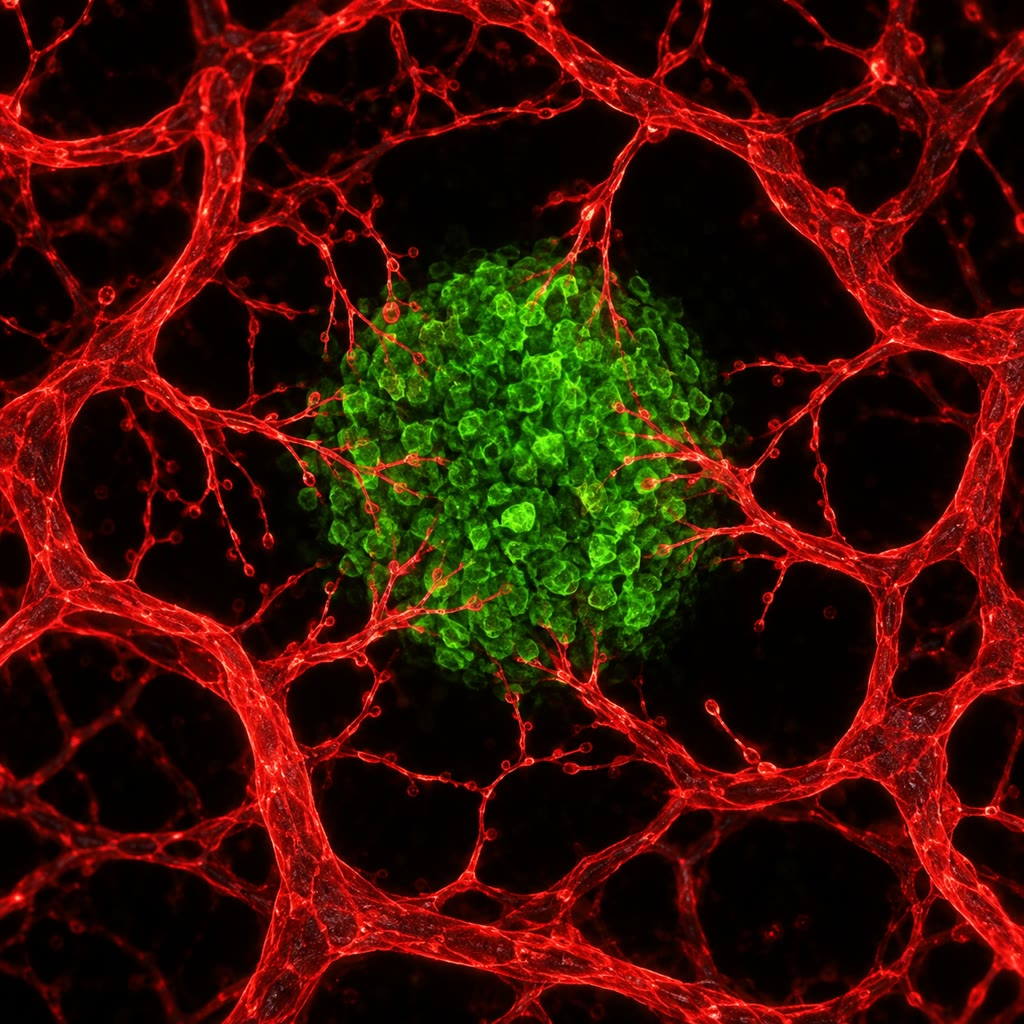
\includegraphics[width=0.36\linewidth]{images/book5/ai/b5-11-angiogenesis.jpg}\hspace{0.04\linewidth}
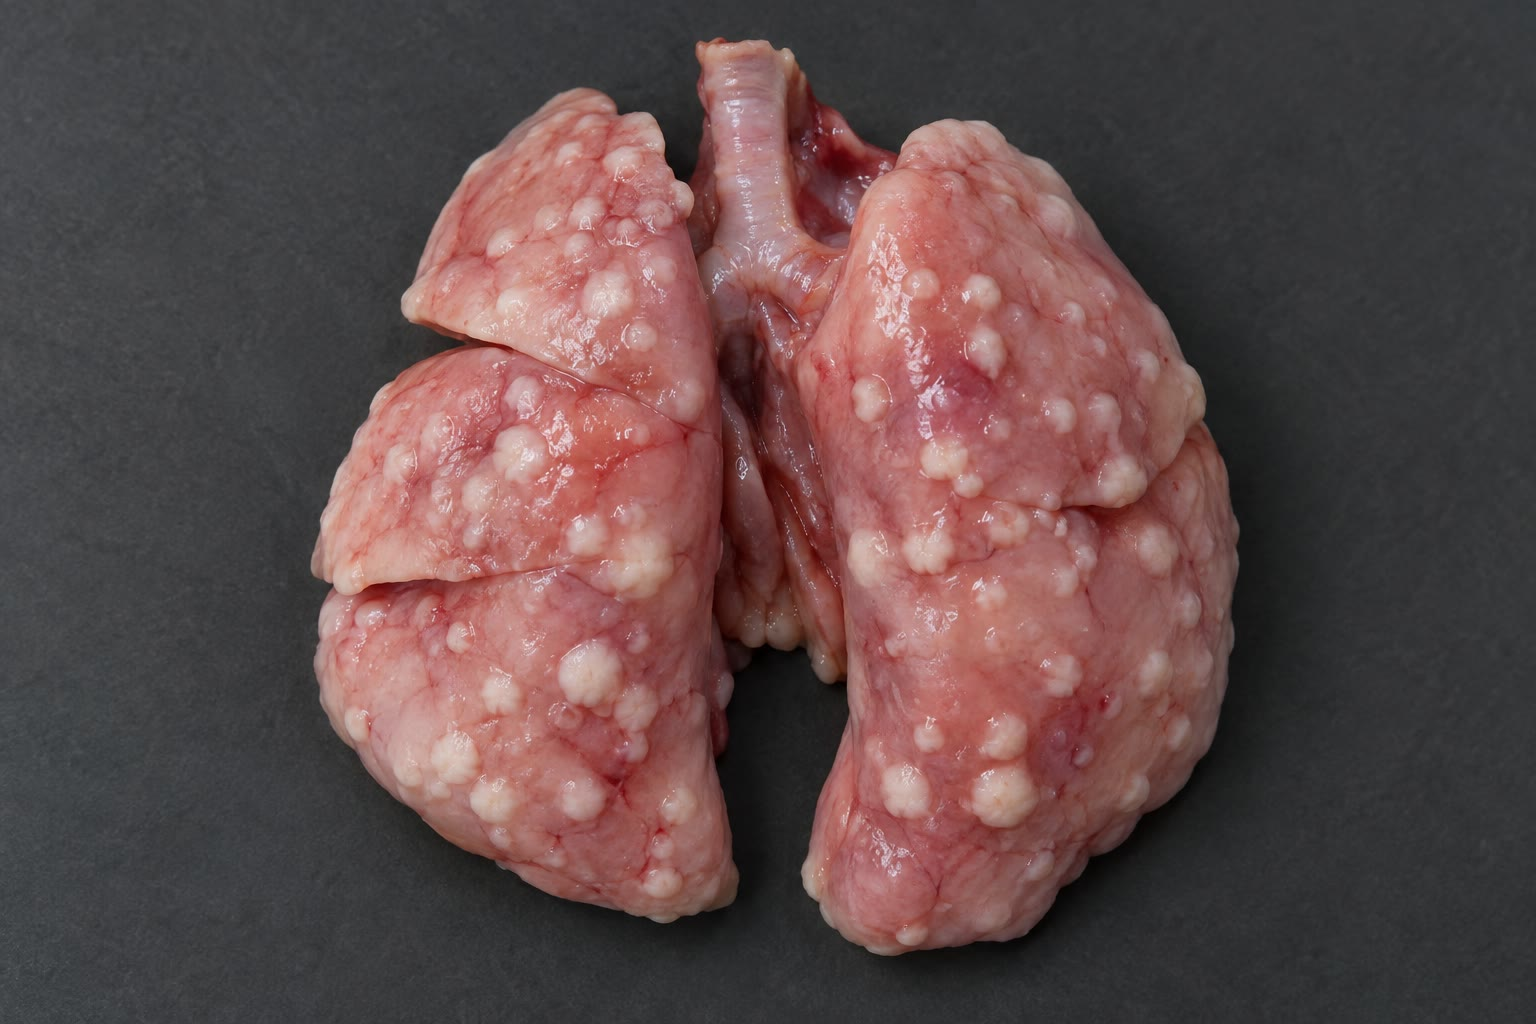
\includegraphics[width=0.54\linewidth]{images/book5/ai/b5-11-metastasis-lung.jpg}

{\small Links: een tumorbolletje (groen) dat nieuwe vaten (rood) uit een
naburig netwerk aantrekt --- angiogenese in kweek. Rechts: een
muizenlong bezaaid met \omterm{def:b3:cancer-biology:hallmarks}{metastasen}, waarbij elke kolonie is gesticht
door één cel die de reis door het bloed overleefde.}
\end{omfigure}

\begin{definition}[Invasie en metastase]\label{def:b3:cancer-biology:metastasis}
\index{invasie}\index{epitheliaal-mesenchymale overgang}\index{zaad en bodem}
Om uit te zaaien moet een carcinoomcel het epitheel verlaten --- haar
celverbindingen en polariteit verliezen en beweeglijkheid verwerven,
een \emph{epitheliaal-mesenchymale overgang} aangedreven door
transcriptiefactoren die normaal in de embryonale ontwikkeling worden
gebruikt --- het basaalmembraan en de matrix met uitgescheiden
proteasen afbreken, de wand van een bloed- of lymfevat oversteken, in
de bloedsomloop overleven (minder dan één op tienduizend doet dat,
gedood door afschuiving, door het ontbreken van hechting en door
natuurlijke doodcellen), zich in een haarvatbed van een ander orgaan
vastzetten, eruit stappen en daar groeien. Waar zij groeit is niet
willekeurig: borstkanker gaat naar bot, long, lever en hersenen,
darmkanker naar de lever, prostaatkanker naar bot --- het \emph{zaad en
de bodem} van Paget uit 1889, deels verklaard door de bloedstroom en
deels door het passen van de cel bij de signalen van het weefsel. Een
verspreide cel kan jaren sluimeren voordat zij groeit, en daarom keren
\omterm{def:b3:cancer-biology:hallmarks}{kankers} een decennium na een schijnbare genezing terug. De \omterm{def:b3:cancer-biology:hallmarks}{metastase}
veroorzaakt negen van de tien sterfgevallen door vaste \omterm{def:b3:cancer-biology:hallmarks}{tumoren}, en zij
is de stap die het minst wordt begrepen.
\end{definition}

\begin{proposition}[Het afweersysteem ontsnappen]\label{prop:b3:cancer-biology:immune}
\index{immuunontwijking}\index{controlepuntremmer}\index{neoantigeen}
De mutaties van een \omterm{def:b3:cancer-biology:hallmarks}{tumor} maken \emph{neoantigenen}, peptiden die geen
enkele normale cel toont, en cytotoxische T-cellen herkennen en doden
tumorcellen --- de reden dat patiënten met een onderdrukte afweer meer
\omterm{def:b3:cancer-biology:hallmarks}{kankers} hebben en de reden dat \omterm{def:b3:cancer-biology:hallmarks}{tumoren} met veel mutaties (melanoom,
long, dikke darm zonder \omterm{prop:b3:dna-repair:fidelity}{mismatchherstel}) het best op immuuntherapie
reageren. Een klinisch merkbare \omterm{def:b3:cancer-biology:hallmarks}{tumor} is er een die is ontsnapt: door
de MHC-moleculen te verliezen die peptiden tonen, door onderdrukkende
factoren uit te scheiden, door regulerende T-cellen aan te trekken, en
vooral door PD-L1 tot expressie te brengen, dat de remmende receptor
PD-1 op T-cellen aangrijpt en hen uitschakelt, dezelfde rem die een
afweerreactie normaal beëindigt
(\cref{ch:b3:adaptive-immunity}). Antilichamen die PD-1 of PD-L1
blokkeren, of de eerdere rem CTLA-4, laten de T-cellen los; bij een
deel van de patiënten --- een vijfde tot de helft, afhankelijk van de
\omterm{def:b3:cancer-biology:hallmarks}{tumor} --- geven zij blijvende remissies van \omterm{def:b3:cancer-biology:hallmarks}{kankers} die onbehandelbaar
waren, en hun bijwerkingen zijn auto-immuniteit, de andere functie van
die rem.
\end{proposition}

\section{Oorzaken en behandelingen}

\begin{proposition}[Oorzaken]\label{prop:b3:cancer-biology:causes}
\index{carcinogeen}\index{oncogeen virus}
\omterm{def:b3:cancer-biology:hallmarks}{Kanker} wordt veroorzaakt door alles wat de snelheid van de
gebeurtenissen uit de stelling of het aantal cellen dat ze loopt
verhoogt. \emph{Chemische carcinogenen}, waarvan de meeste na
activering door de lever mutageen zijn: de zeventig carcinogenen van
tabaksrook, die een derde van de sterfgevallen door \omterm{def:b3:cancer-biology:hallmarks}{kanker} veroorzaken
en het risico op longkanker vijftien- tot vijfentwintigvoudig verhogen;
aflatoxine uit beschimmeld graan; asbest, dat geen mutageen is maar een
chronische prikkel. \emph{Straling}: ultraviolet licht voor de huid (de
dimeren van \cref{ch:b3:dna-repair}), ioniserende straling voor
leukemie, schildklier en borst. \emph{Infecties}, een zesde van de
\omterm{def:b3:cancer-biology:hallmarks}{kankers} wereldwijd: de papillomavirussen, waarvan de eiwitten E6 en E7
\omterm{def:b3:cancer-biology:genes}{p53} vernietigen en Rb uitschakelen en die vrijwel alle
baarmoederhalskankers veroorzaken (een vaccin voorkomt ze nu); de
hepatitis-B- en -C-virussen bij leverkanker; het epstein-barrvirus bij
lymfomen; \emph{Helicobacter pylori} bij maagkanker, via decennia van
ontsteking. \emph{Geërfde mutaties} in een tumorsuppressor, de eerste
treffer bij de geboorte, bij zo'n \qty{5}{\%} van de \omterm{def:b3:cancer-biology:hallmarks}{kankers}. En het
toeval: de meeste mutaties in een \omterm{def:b3:cancer-biology:hallmarks}{tumor} kwamen voort uit de gewone
fouten van de replicatie, zodat de weefsels die zich het meest delen
--- dikke darm, huid, bloed --- de meeste \omterm{def:b3:cancer-biology:hallmarks}{kankers} hebben, en het risico
stijgt met de leeftijd wat men ook doet.
\end{proposition}

\begin{theorem}[Waarom één geneesmiddel faalt en twee misschien niet]\label{thm:b3:cancer-biology:goldie-coldman}
\index{model van Goldie--Coldman}\index{resistentie tegen geneesmiddelen}\index{combinatietherapie}
Laat een \omterm{def:b3:cancer-biology:hallmarks}{tumor} van $N$ cellen door opeenvolgende delingen uit één cel
zijn ontstaan, en laat een mutatie die resistentie tegen een gegeven
geneesmiddel geeft met snelheid $\mu$ per celdeling optreden. Dan is de
kans dat de \omterm{def:b3:cancer-biology:hallmarks}{tumor} \emph{geen} resistente cel bevat wanneer de
behandeling begint ongeveer
\[
P_{0} \approx e^{-\mu N},
\]
zodat voor $\mu N \gg 1$ de resistentie vrijwel zeker al bestaat. Voor
twee geneesmiddelen met onafhankelijke resistentiemechanismen ontstaat
een cel die tegen beide bestand is met een snelheid van ongeveer
$\mu_{1}\mu_{2}$ per deling, en is $P_{0}
\approx e^{-\mu_{1}\mu_{2}N}$: met $N = 10^{9}$ en $\mu = 10^{-7}$ staat
één geneesmiddel gemiddeld tegenover $\mu N = 100$ resistente klonen,
en twee geneesmiddelen tegenover een kans van $10^{-5}$ dat er ook maar
één dubbel resistente cel bestaat.
\end{theorem}
\begin{proof}[Gedeeltelijk bewijs]
Van $1$ tot $N$ cellen groeien kost in totaal ongeveer $N$ delingen
(een boom met $N$ bladeren heeft $N - 1$ inwendige knopen). Wordt er bij
elke deling met kans $\mu$ een resistente cel gemaakt en sterven haar
nakomelingen in eerste benadering niet en groeien zij de rest niet
voorbij, dan is het aantal resistentiegebeurtenissen poissonverdeeld
met gemiddelde $\mu N$, en is de kans op geen enkele $e^{-\mu N}$.
Onafhankelijke mechanismen vermenigvuldigen de kansen per deling. De
benadering gaat eraan voorbij dat vroege mutanten grotere resistente
klonen achterlaten --- de volledige verdeling is die van Luria en
Delbrück, behandeld in het boek van jaar~2 --- maar de kans op
\emph{geen} mutant, die bepaalt of de \omterm{def:b3:cancer-biology:hallmarks}{tumor} te genezen is, is precies
de poissonterm.
\end{proof}

\begin{example}[Behandelingen en hun logica]\label{ex:b3:cancer-biology:therapy}
Chirurgie en radiotherapie halen een plaatselijke \omterm{def:b3:cancer-biology:hallmarks}{tumor} weg of doden
hem; straling doodt met \omterm{def:b3:dna-repair:lesions}{dubbelstrengsbreuken}, en het opdelen in
dagelijkse doses laat normaal weefsel ertussen herstellen
(\cref{ch:b3:dna-repair}). Cytotoxische chemotherapie --- alkylerende
stoffen, antimetabolieten, vergiften van de \omterm{def:b3:cytoskeleton-motility:filaments}{microtubuli}, remmers van
topo-isomerasen --- doodt delende cellen van welke soort ook,
tumorcellen iets meer, en volgt een \emph{logdodingswet}: elke kuur
doodt een vast deel, zeg \qty{99}{\%}, zodat zes kuren $10^{12}$ cellen
tot één terugbrengen, en diezelfde zes kuren nodig zijn of de \omterm{def:b3:cancer-biology:hallmarks}{tumor} nu
groot of klein is; het haar, de darm en het beenmerg van de patiënt,
die zich ook delen, bepalen de dosis. Gerichte therapie valt een
beschadiging aan waarvan de \omterm{def:b3:cancer-biology:hallmarks}{tumor} afhangt: imatinib blokkeert het
BCR--ABL-kinase en maakte van de chronische myeloïde leukemie een
chronische in plaats van een dodelijke ziekte; trastuzumab bindt HER2;
de PARP-remmers, de Cdk4/6-remmers en venetoclax uit eerdere
hoofdstukken benutten elk één defect. De immuuntherapie laat de
T-cellen los. En de stelling zegt hoe zij moeten worden gebruikt: in
combinatie, vroeg, wanneer $N$ het kleinst is --- en dat is wat
aanvullende chemotherapie na een operatie doet --- en met
geneesmiddelen waarvan de resistentiemechanismen elkaar niet
overlappen. De \omterm{def:b3:cancer-biology:hallmarks}{tumor} is een evoluerende populatie, en de behandeling is
selectie.
\end{example}

\begin{omfigure}
\begin{tikzpicture}
\begin{axis}[
  width=0.7\linewidth, height=5.6cm,
  axis x line=bottom, axis y line=left,
  xmin=0, xmax=8, ymin=1, ymax=1e13, ymode=log,
  xlabel={kuren chemotherapie}, ylabel={tumorcellen},
  xlabel style={font=\small, at={(axis description cs:0.5,-0.12)}, anchor=north},
  ylabel style={font=\small},
  tick label style={font=\small}, xtick={0,2,4,6,8},
  clip=false,
]
\addplot[very thick, omDef, mark=*, mark size=1.2pt] coordinates {(0,1e12) (1,1e10) (2,1e8) (3,1e6) (4,1e4) (5,1e2) (6,1)};
\addplot[very thick, omThm, mark=*, mark size=1.2pt] coordinates {(0,1e12) (1,1.01e10) (2,1.02e8) (3,1.04e6) (4,1.1e4) (5,200) (6,300) (7,600) (8,1200)};
\addplot[dashed, gray, domain=0:8, samples=2] {1e9};
\node[font=\scriptsize, gray, anchor=south west] at (axis cs:0.2,1.3e9) {aantoonbaar, $10^{9}$};
\node[font=\scriptsize, omDef, anchor=south west] at (axis cs:0.3,1e4) {\qty{99}{\%} gedood per kuur};
\node[font=\scriptsize, omThm, anchor=south west] at (axis cs:5.2,3e3) {één resistente cel bij aanvang: terugkeer};
\end{axis}
\end{tikzpicture}

{\small De logdodingswet. Elke kuur doodt hetzelfde deel van de cellen,
zodat de \omterm{def:b3:cancer-biology:hallmarks}{tumor} per kuur met een vast aantal decaden krimpt en lang
onaantoonbaar is voordat hij weg is (blauw); één enkele reeds
aanwezige resistente cel overleeft elke kuur en groeit weer aan (rood).}
\end{omfigure}

\begin{remark}[Wat er is veranderd]\label{rem:b3:cancer-biology:changed}
De helft van alle patiënten bij wie in een rijk land \omterm{def:b3:cancer-biology:hallmarks}{kanker} wordt
vastgesteld overleeft nu tien jaar, tegen een kwart in 1970. De winst
kwam van preventie (tabak, vaccins tegen hepatitis en
papillomavirus, het opsporen van poliepen en afwijkingen aan de
baarmoederhals), van eerdere opsporing, en van behandelingen die uit de
biologie van dit hoofdstuk volgen --- de combinatiechemotherapie die de
meeste leukemieën bij kinderen en de teelbalkankers geneest, de
gerichte geneesmiddelen, en de immuuntherapieën. Wat niet is veranderd
is de uitgezaaide ziekte, die de biologie verklaart maar nog niet
geneest; de volgende winst zal komen van de \omterm{def:b3:cancer-biology:hallmarks}{tumor} te behandelen als wat
hij is: een populatie die evolueert onder de selectie die de
behandeling oplegt.
\end{remark}

\section{Opgaven}

\begin{exercise}[$\star$]\label{exo:b3:cancer-biology:1}
Onderscheid een \omterm{def:b3:cancer-biology:genes}{oncogen} van een \omterm{def:b3:cancer-biology:genes}{tumorsuppressorgen} naar mechanisme,
naar het aantal allelen dat moet veranderen, en met van elk twee
voorbeelden.
\end{exercise}

\begin{exercise}[$\star$]\label{exo:b3:cancer-biology:2}
Noem de \omterm{def:b3:cancer-biology:hallmarks}{kenmerken van kanker} en bij elk één gen uit dit of een eerder
hoofdstuk waarvan de verandering dat kenmerk levert.
\end{exercise}

\begin{exercise}[$\star$]\label{exo:b3:cancer-biology:3}
Wat nam Knudson waar over het erfelijke en het sporadische
retinoblastoom, en wat leidde hij daaruit af?
\end{exercise}

\begin{exercise}[$\star$]\label{exo:b3:cancer-biology:4}
Leg de \omterm{met:b3:cancer-biology:ames}{amestest} uit en waarom er een leverextract wordt toegevoegd.
\end{exercise}

\begin{exercise}[$\star\star$]\label{exo:b3:cancer-biology:5}
De incidentie van een \omterm{def:b3:cancer-biology:hallmarks}{kanker} is $2\times 10^{-5}$ per jaar op leeftijd
$40$ en $2\times 10^{-3}$ op leeftijd $80$. Schat de exponent van de
machtswet in de leeftijd en het aantal snelheidsbepalende
gebeurtenissen dat die suggereert.
\end{exercise}

\begin{exercise}[$\star\star$]\label{exo:b3:cancer-biology:6}
Bereken met \cref{prop:b3:cancer-biology:oxygen} bij $D =
\qty{2e-9}{m^2/s}$ en $c_{0} = \qty{0.05}{mol/m^3}$ de waarde van $L$
voor weefsel dat \qty{0.01}{mol/m^3/s} verbruikt en voor een \omterm{def:b3:cancer-biology:hallmarks}{tumor} die
driemaal zoveel verbruikt. Waarom wordt een snel groeiende \omterm{def:b3:cancer-biology:hallmarks}{tumor} eerder
necrotisch?
\end{exercise}

\begin{exercise}[$\star\star$]\label{exo:b3:cancer-biology:7}
Een \omterm{def:b3:cancer-biology:hallmarks}{tumor} van $10^{11}$ cellen wordt behandeld met een middel dat per
kuur \qty{99.9}{\%} doodt. Hoeveel kuren zijn er nodig om hem onder één
cel te brengen? Waarom is de \omterm{def:b3:cancer-biology:hallmarks}{tumor} na twee kuren onaantoonbaar hoewel
er nog $10^{5}$ cellen over zijn, en wat betekent dat voor het staken
van de behandeling?
\end{exercise}

\begin{exercise}[$\star\star$]\label{exo:b3:cancer-biology:8}
Leg uit waarom een mutatie in EGFR en een mutatie in KRAS zelden in
dezelfde longtumor worden gevonden, en waarom een \omterm{def:b3:cancer-biology:hallmarks}{tumor} die met een
EGFR-remmer wordt behandeld vaak terugkeert met een mutatie in KRAS.
\end{exercise}

\begin{exercise}[$\star\star$]\label{exo:b3:cancer-biology:9}
De papillomaviruseiwitten E6 en E7 schakelen \omterm{def:b3:cancer-biology:genes}{p53} en Rb uit. Leg uit hoe
dit baarmoederhalskanker aandrijft, waarom het decennia kost, en waarom
een vaccin dat vóór de seksuele activiteit wordt gegeven het voorkomt.
\end{exercise}

\begin{exercise}[$\star\star\star$]\label{exo:b3:cancer-biology:10}
Breid het argument van Armitage en Doll uit zodat elke treffer zijn
kloon met een factor $g$ mag uitbreiden voordat de volgende komt: laat
zien dat de incidentie dezelfde macht van $t$ heeft maar een voorfactor
die met $g^{k-1}$ is vermenigvuldigd, en bespreek waarom de uit een
leeftijdscurve gefitte $k$ een bovengrens is voor het aantal
aandrijvers.
\end{exercise}

\begin{exercise}[$\star\star\star$]\label{exo:b3:cancer-biology:11}
Vergelijk met \cref{thm:b3:cancer-biology:goldie-coldman} (a) het
behandelen van een \omterm{def:b3:cancer-biology:hallmarks}{tumor} van $10^{9}$ cellen met middel A gedurende zes
kuren en daarna met middel B gedurende zes, en (b) A en B vanaf het
begin samen geven, wanneer $\mu_{A} =
\mu_{B} = 10^{-7}$. Bereken $P_{0}$ voor elke strategie en leg uit
waarom een vroege combinatie de regel is.
\end{exercise}

\begin{exercise}[$\star\star\star$]\label{exo:b3:cancer-biology:12}
De paradox van Peto: een olifant heeft honderd keer zoveel cellen als
een mens en leeft even lang, en toch heeft hij niet meer \omterm{def:b3:cancer-biology:hallmarks}{kanker}. Zeg
met de stelling van dit hoofdstuk wat de naïeve verwachting is, en stel
twee mechanismen voor waarmee grote dieren het probleem opgelost kunnen
hebben (de olifant heeft twintig kopieën van \emph{TP53}).
\end{exercise}

\section{Vraagstuk: de rekenkunde van een tumor}

\begin{problem}[{Weekendvraagstuk --- een tumor uit één cel gegroeid en
tot aan de ontdekking in de tijd gezet, zijn leeftijdscurve gelezen op
het aantal treffers, zijn zuurstofvoorziening en necrotische kern
berekend, en zijn behandeling gepland tegen de zekerheid van
resistentie, met als besluit het aantal jaren tot de ontdekking, de
diepte van levende tumor rond een vat en de kans dat een combinatie
geneest}]
\label{pb:b3:cancer-biology:1}
Gegevens: een tumorcel heeft een volume van \qty{1000}{\micro m^3}; de
verdubbelingstijd is \qty{100}{dagen}; de ontdekking gebeurt bij
\qty{1}{cm^3}; de dodelijke last is \qty{1}{kg}. Leeftijdscurve:
incidentie $1\times 10^{-5}$ per jaar op $30$ en $3\times
10^{-3}$ op $80$. Zuurstof: $D = \qty{2e-9}{m^2/s}$, $c_{0} =
\qty{0.05}{mol/m^3}$, $q = \qty{0.03}{mol/m^3/s}$ in de \omterm{def:b3:cancer-biology:hallmarks}{tumor}; de
haarvaten in een doorbloede \omterm{def:b3:cancer-biology:hallmarks}{tumor} liggen \qty{150}{\micro m} uit
elkaar. Behandeling: elke kuur doodt \qty{99}{\%}; de mutatiesnelheid
voor resistentie is $10^{-7}$ per deling per middel; er is een kuur om
de drie weken; de \omterm{def:b3:cancer-biology:hallmarks}{tumor} groeit tussen de kuren met dezelfde
verdubbelingstijd aan.

\medskip
\noindent\textbf{Deel I --- Groei.}
\begin{enumerate}
  \item Hoeveel cellen zitten er in \qty{1}{cm^3}? Hoeveel
        verdubbelingen vanaf één cel?
  \item Hoeveel jaar van de stichtende cel tot de ontdekking?
  \item Hoeveel verdubbelingen, en jaren, van de ontdekking tot de
        dodelijke last? Vergelijk de twee tijdvakken.
  \item Veel \omterm{def:b3:cancer-biology:hallmarks}{tumoren} worden bij \qty{1}{cm^3} ontdekt maar groeiden pas
        vijf jaar. Wat moet er dan waar zijn geweest van de
        verdubbelingstijd in het begin, of van de groeiwet?
  \item Slechts een deel $f$ van de cellen in een \omterm{def:b3:cancer-biology:hallmarks}{tumor} deelt zich op
        enig moment (de groeifractie), en een deel sterft. Als cellen
        hun cyclus in \qty{2}{dagen} doorlopen maar de \omterm{def:b3:cancer-biology:hallmarks}{tumor} zich in
        $100$ verdubbelt, wat zegt dat dan over het evenwicht tussen
        geboorte en dood?
  \item Waarom spaart dezelfde logdodingschemotherapie een traag
        groeiende \omterm{def:b3:cancer-biology:hallmarks}{tumor} meer dan een snelle, en groeit de snelle toch
        sneller tussen de kuren aan?
\end{enumerate}

\medskip
\noindent\textbf{Deel II --- Treffers.}
\begin{enumerate}[resume]
  \item Bereken uit de twee incidenties de exponent $k - 1$ van de
        leeftijdscurve en het bijbehorende aantal gebeurtenissen $k$.
  \item Als elke gebeurtenis met $u = 10^{-6}$ per cel per jaar
        optreedt in $N = 10^{8}$ vatbare cellen, wat voorspelt de
        stelling dan voor het cumulatieve risico op leeftijd $70$ met
        de gevonden $k$? Is dat aannemelijk? Wat ontbreekt er?
  \item Doe hetzelfde met een klonale uitbreiding met een factor
        $g = 100$ na elk van de eerste $k - 1$ treffers, met
        \cref{exo:b3:cancer-biology:10}.
  \item Een draagster erft één treffer. Met welke factor stijgt haar
        incidentie op leeftijd $40$, als de overige snelheden
        onveranderd blijven? (Vergelijk $(ut)^{k-1}$ met $(ut)^{k}$ bij
        $t = 40$.)
  \item Roken vermenigvuldigt $u$ voor één van de gebeurtenissen met
        $10$. Met welke factor stijgt de incidentie als die gebeurtenis
        er één van $k$ is, en als het er twee zijn?
  \item Leg uit waarom stoppen met roken op vijftigjarige leeftijd het
        risico op longkanker onder dat van een doorrokende brengt, maar
        nooit tot dat van iemand die nooit heeft gerookt.
\end{enumerate}

\medskip
\noindent\textbf{Deel III --- Aanvoer.}
\begin{enumerate}[resume]
  \item Bereken de indringdiepte $L$ van de zuurstof in de \omterm{def:b3:cancer-biology:hallmarks}{tumor}.
  \item Een bolletje zonder vaten: wat is de grootste doorsnede waarbij
        elke cel van zuurstof is voorzien? Hoe dik is de levende rand
        van een bolletje van \qty{2}{mm}, en welk deel van zijn volume
        leeft?
  \item Is in een doorbloede \omterm{def:b3:cancer-biology:hallmarks}{tumor} met haarvaten op \qty{150}{\micro m}
        van elkaar elke cel van zuurstof voorzien? Welke cellen zijn
        hypoxisch, en waarom doet dat ertoe voor de radiotherapie
        (zuurstof legt de stralingsschade vast) en voor de selectie van
        cellen met mutant \omterm{def:b3:cancer-biology:genes}{p53}?
  \item Een geneesmiddel halveert de dichtheid van de haarvaten in de
        \omterm{def:b3:cancer-biology:hallmarks}{tumor}. Herbereken de afstand en zeg wat er gebeurt met de
        cellen halverwege tussen de vaten.
  \item Hypoxische cellen schakelen over op de glycolyse en maken
        \qty{2}{ATP} per glucose in plaats van $30$. Met welke factor
        moeten zij hun glucoseopname verhogen om hun ATP-aanvoer op
        peil te houden, en hoe wordt dat benut bij het afbeelden van
        \omterm{def:b3:cancer-biology:hallmarks}{tumoren}?
  \item Leg uit waarom antiangiogene therapie op zichzelf zelden
        geneest maar de chemotherapie wel kan helpen de \omterm{def:b3:cancer-biology:hallmarks}{tumor} te
        bereiken.
\end{enumerate}

\medskip
\noindent\textbf{Deel IV --- Behandeling.}
\begin{enumerate}[resume]
  \item Een \omterm{def:b3:cancer-biology:hallmarks}{tumor} van \qty{1}{cm^3} wordt met één middel behandeld.
        Hoeveel kuren brengen hem onder één cel, als aangroei en
        resistentie buiten beschouwing blijven?
  \item Tussen de kuren (drie weken) groeien de overlevenden aan. Met
        welke factor? Herbereken de nettododing per cyclus en het
        aantal cycli dat nodig is.
  \item Bereken het verwachte aantal cellen dat bij het begin van de
        behandeling tegen het middel bestand is, en de kans dat er geen
        enkele is.
  \item Er worden twee middelen met onafhankelijke mechanismen samen
        gegeven. Wat is de kans dat er bij het begin geen dubbel
        resistente cel bestaat? En bij een \omterm{def:b3:cancer-biology:hallmarks}{tumor} van $10^{12}$ cellen?
  \item Aanvullende therapie wordt na een operatie gegeven, wanneer er
        misschien $10^{6}$ cellen onopgemerkt achterblijven. Herbereken
        de kansen voor één en voor twee middelen, en formuleer de les.
  \item Een immuuntherapie wekt T-cellen op die elke cel doden die een
        neoantigeen toont. Waarom is resistentie daartegen een ander
        probleem dan resistentie tegen een kinaseremmer, en op welke
        \omterm{def:b3:cancer-biology:hallmarks}{tumoren} zou zij volgens de stelling het best moeten werken?
  \item Vat samen: het aantal jaren van de stichtende cel tot de
        ontdekking (vraag~2), de diepte van levende \omterm{def:b3:cancer-biology:hallmarks}{tumor} rond een vat
        (vraag~13), en de kans dat de combinatie van twee middelen in
        een \omterm{def:b3:cancer-biology:hallmarks}{tumor} van \qty{1}{cm^3} geen resistente cel tegenkomt
        (vraag~22).
\end{enumerate}
\end{problem}
